\chapter{XenoFlow Loadbalancer}
\label{cha:implementation}
Ziel dieser Bachelorarbeit war es, einen möglichst hardwarebeschleunigten Lastverteiler zu entwickeln. Dazu wurde das DOCA Flow Framework verwendet, da die zur Verfügung stehende Netzwerkkarte eine BlueField-3 ist. Im folgenden Kapitel wird ein Überblick über die Entwicklung mit DOCA Flow gegeben und es werden die Kernelemente des XenoFlow LoadBalancers vorgestellt. XenoFlow ist nicht für Produktionsumgebungen gedacht, sondern soll vielmehr ein Proof-of-Concept darstellen und einen speziellen Anwendungsfall demonstrieren. XenoFlow ist aktuell auch nur in der Lage, UDP-Pakete zu verarbeiten. Diese Entscheidung ist damit zu begründen, dass eine beispielsweise eine TCP-Verbindung mehr Umstände beinhaltet, die berücksichtigt werden müssten. Zunächst soll aber nur die Machbarkeit und die allgemeine Performance beurteilt werden. Der komplette Quellcode von XenoFlow ist unter der MIT veröffentlicht und unter den weiter unten angegebenen Git-Repositories verfügbar.
\section{Entwicklung}
NVidia stellt eine Menge von Beispielapplikationen für die verschiedenen DOCA Frameworks und Libraries zur Verfügung. Der erste Teil der Entwicklung dieses Lastverteilers bestand also darin, eine Wissensbasis für DOCA und hier im Speziellen DOCA Flow aufzubauen. Darunter fielen allerdings gerade zu Beginn der Entwicklung viele Probleme auf. Das wohl größte Problem ist, dass DOCA und damit auch DOCA Flow nur mit einer sehr schlechten Dokumentation ausgestattet sind. So werden die meisten Teilbereiche zwar angesprochen, aber leider meist nicht im Detail erläutert. Außerdem finden sich häufig widersprüchliche Aussagen in der Dokumentation. Zuweilen werden auch Abkürzungen verwendet, die nirgends klar definiert werden und somit den Leser in völligem Unwissen darüber lassen, was sie zu bedeuten haben sollen. Oftmals gewinnt man als Leser den Eindruck, es handele sich um eine relativ diffus zusammengeworfene Wissensbasis, die keiner Qualitätskontrolle unterlaufen ist. Es schienen mehrere Entwicklungsteams an dem Verfassen der Dokumentation beteiligt gewesen zu sein, da oftmals stark unterschiedliche Programmierstile verwendet wurden. Dies führt abermals oftmals zur Verwirrung auf Seiten des Lesers. Dazu sei erwähnt, dass etwaige Enterprise-Produkte wie in diesem Fall BlueField, so vermarktet werden, dass die eigentliche Hardware nur einen Teil der Dienstleistung umfasst. Oftmals werden dazu noch Schulungen gebucht, die das beteiligte Entwicklungspersonal in der Benutzung der Plattform unterweisen sollen. 

Diese Möglichkeiten sind aus finanziellen als auch personaltechnischen Gründen nicht an einer deutschen Hochschule gegeben. Somit ist es dem auf dem Gebiet arbeitenden Personal selbst überlassen, Informationen auf dem Gebiet zu gewinnen. Auch das NVidia-Forum, welches ein spezielles Unterforum für die BlueField-Familie besitzt, stellte sich als nicht besonders informativ heraus. Bei einer Anfrage wird entweder nicht geantwortet oder auf eine generische Support-Email-Adresse verwiesen. Wendet man sich an besagte Adresse, soll ein Zertifikat vorgelegt werden, ehe man mit einem tatsächlichen Entwickler Kontakt aufnehmen kann.\newline
Bei den ersten Experimenten auf der BlueField-3 war es zunächst nicht möglich, den Netzwerkverkehr vollständig auf der spezialisierten Hardware zu verarbeiten. Sobald Paketlast entstand, war die Performance an einen einzigen ARM-Kern gebunden und es konnten nur sehr schlechte Verarbeitungsraten erzielt werden. Erst als der Open vSwitch auf der BlueField selbst wie folgt konfiguriert wurde
\begin{minted}{bash}
ovs-ofctl add-flow br0 "in_port=1,actions=output:2"
\end{minted}
verschwand die Last auf den ARM-Kernen und der Verkehr war somit komplett hardwarebeschleunigt.
\subsection{Modify Header und Shared Counter}
\begin{figure}
    \centering
    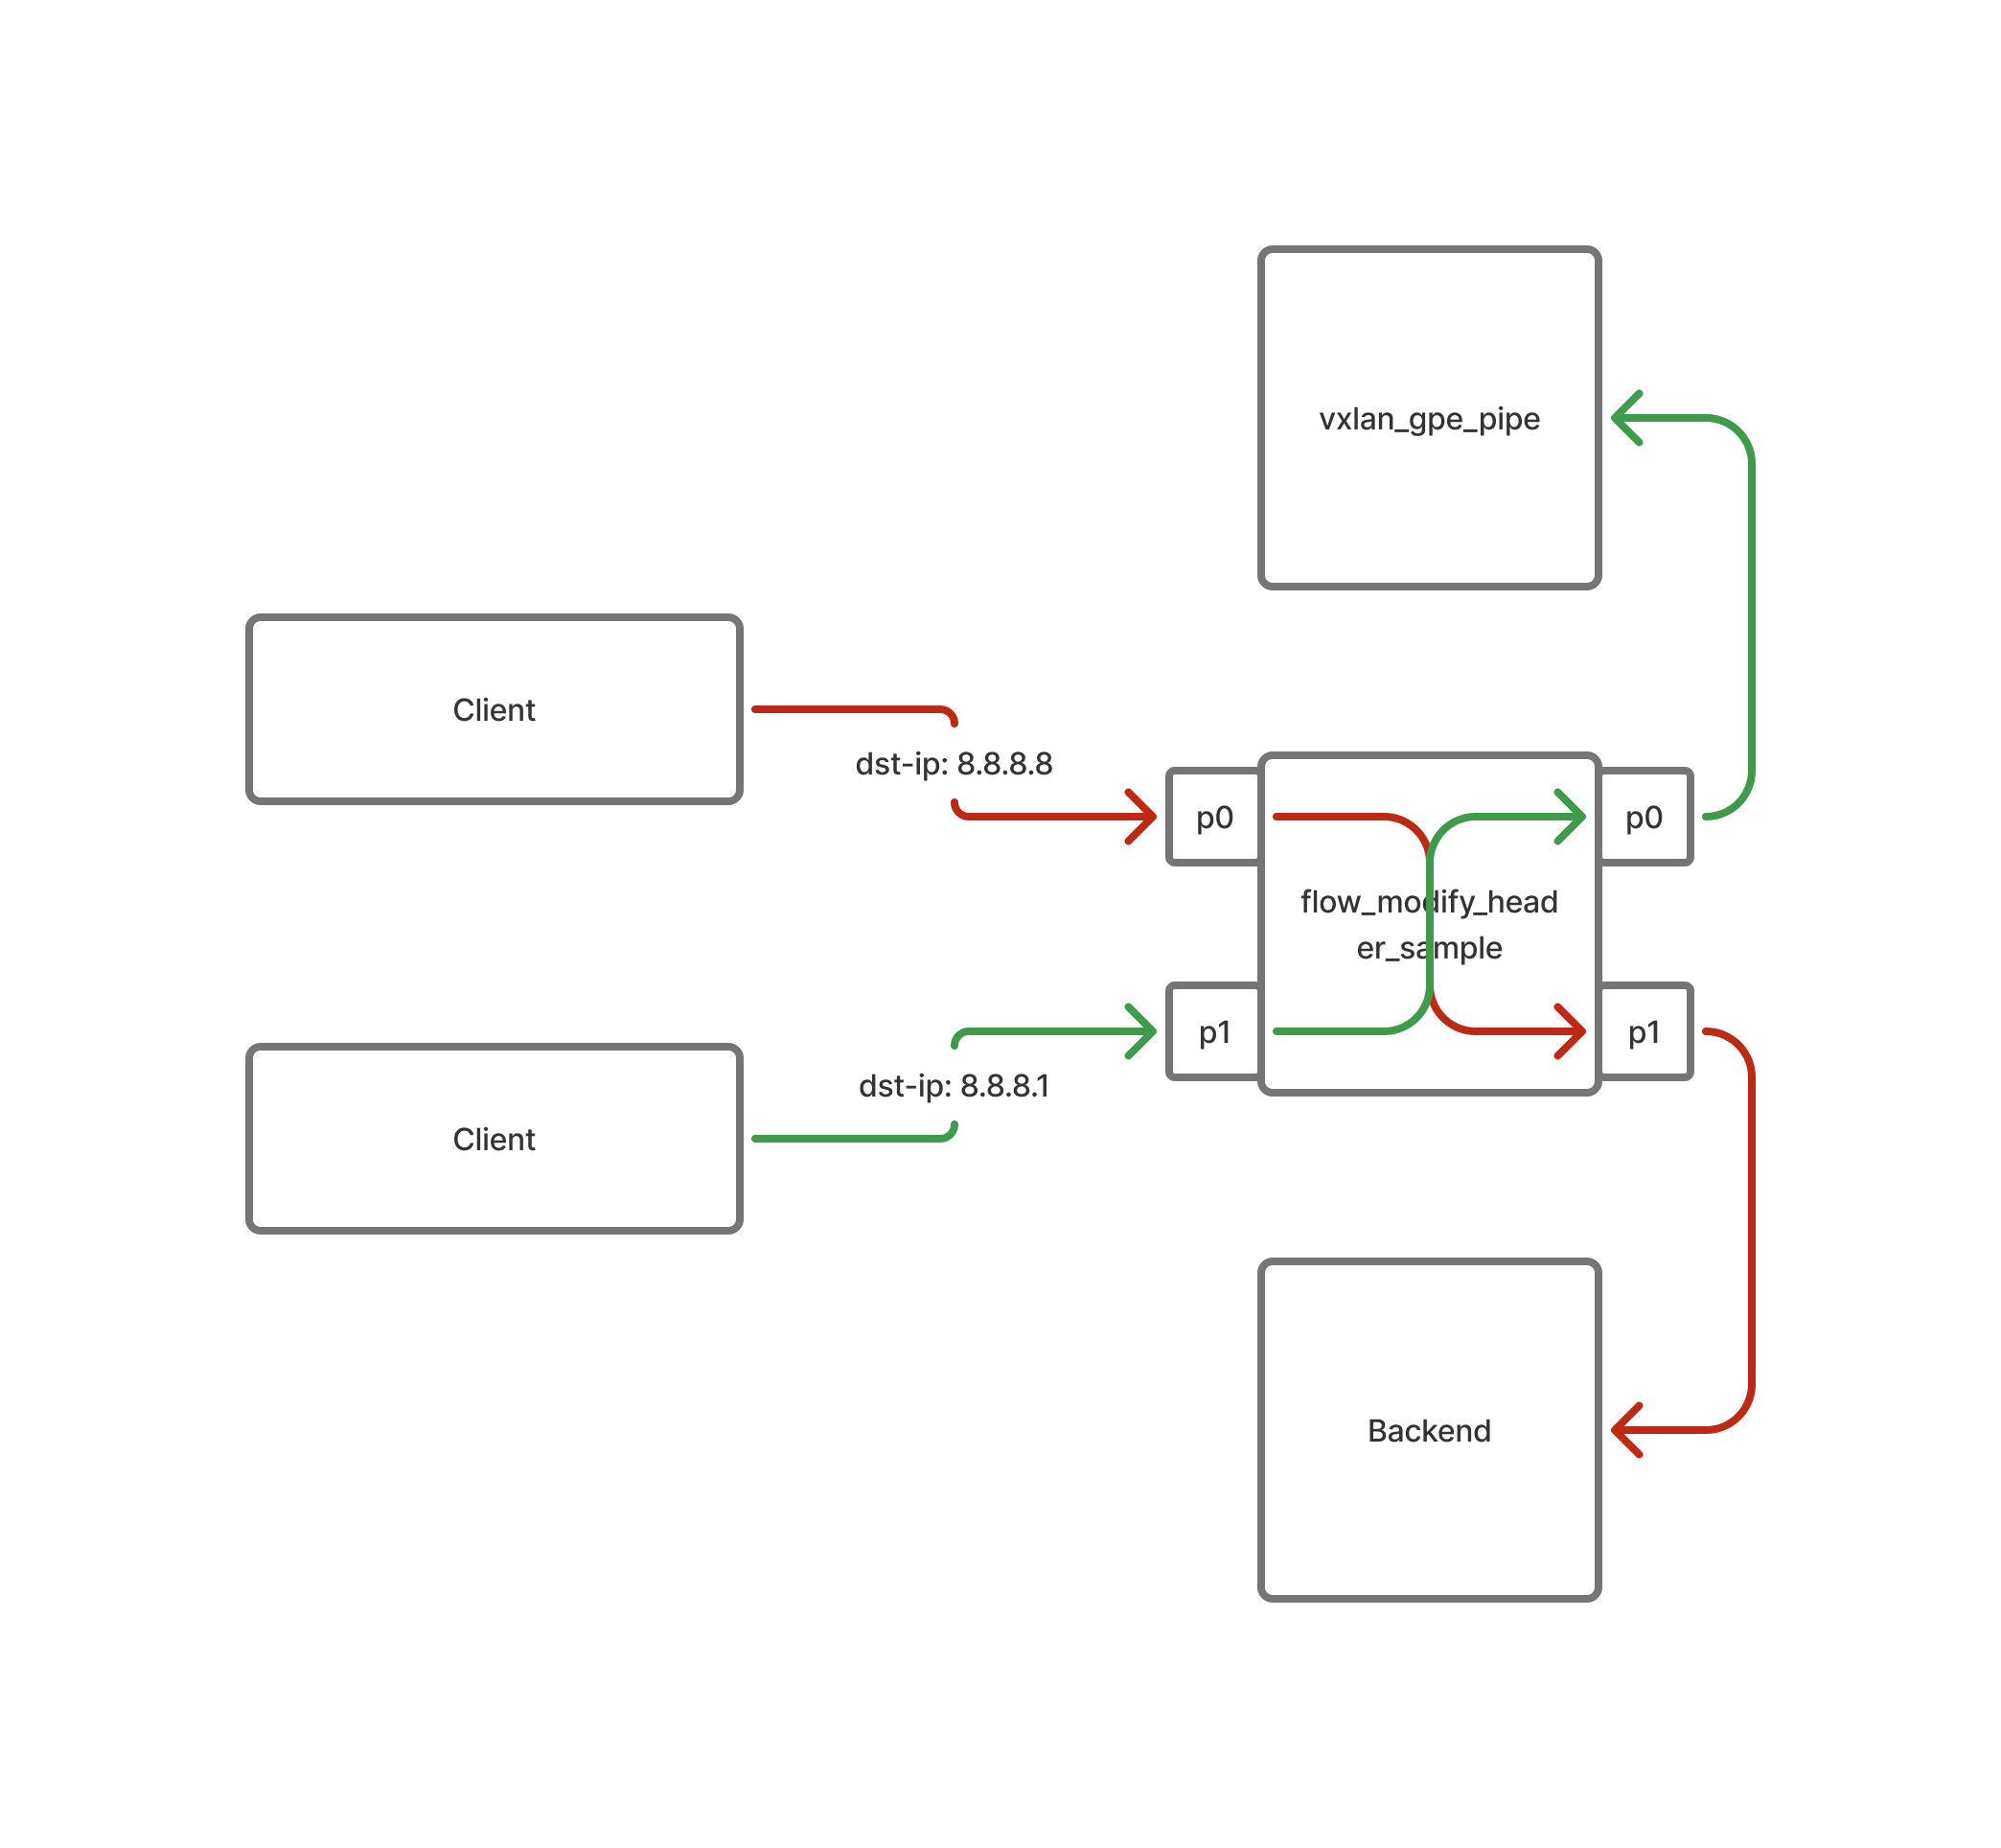
\includegraphics[width=0.8\linewidth]{images/modify_header.png}
    \caption{Flow Modify Header Sample Aufbau}
    \label{fig:enter-label}
\end{figure}
Zu Beginn der Entwicklung wurde auf der Beispielapplikation flow\_modify\_header\_sample.c aufgebaut. Das besagte Beispielprojekt beschreibt eine Anwendung, in der Netzwerkverkehr auf das bestimmte Destination-IP-Feld mit der IP 8.8.8.8 gematcht wird und daraufhin die MAC-Adresse mittels Action geändert wird. Dieser Ansatz ist für die Implementierung eines Load Balancers von großem Interesse. Grund dafür ist, dass ein Netzwerkpaket so manipuliert werden kann, dass es den mit der MAC-Adresse spezifizierten Rechner erreichen kann, dort dann aber eine Modifikation der MAC-Adresse vorgenommen wird, damit das Paket an ein dediziertes Backend weitergeleitet wird. Zusätzlich wurde noch die Beispielapplikation flow\_shared\_counter\_sample.c untersucht. In dieser wird ein Beispiel gegeben, wie von der BlueField erfasste Monitoring-Daten abgerufen werden können, um Informationen über den aktuellen Datenverkehr erhalten zu können. Dies ist, sofern es wirklich Hardwareeinheiten sind, nicht trivial, da es keinen Speicherbereich oder Ähnliches gibt, auf den zugegriffen werden kann, um Daten zu erhalten. DOCA stellt dafür eine Funktion bereit:
\begin{minted}{c}
int doca_flow_shared_resources_query(DOCA_FLOW_SHARED_RESOURCE_COUNTER,
							shared_counter_ids,
							query_results_array,
							nb_ports);
\end{minted}
 Laut der Dokumentation können so mehrere Entries auf den Counter zugreifen bzw. diesen erhöhen. Der gesamte Prozess ist somit vergleichbar mit Thread-Safety bei parallelen Programmen, abgebildet in der DOCA Flow-Semantik mit Flow Entries.

In Abbildung 6.1 ist dargestellt, wie zwei Clients jeweils ein Paket mittels genauer MAC-Adresse an die modify header Applikation schicken. Der rote Pfad beschreibt dabei ein Paket, welches von der ersten Pipe gefangen wird. Daraufhin wird die entsprechende Source MAC-Adresse bearbeitet. Der grüne Pfad beschreibt hingegen ein Paket, welches nicht von der ersten Pipe und deren Entries gefangen wurde. Es wird somit als Miss klassifiziert und in der spezifischen Applikation in eine andere Pipe weitergeleitet. Diese hat im Beispiel nicht für diese Arbeit relevante weitere Operationen in bestimmten Entries definiert. Alle von einem bestimmten Hardwareport der BlueField verarbeiteten Pakete werden an den jeweils anderen Hardwareport weitergeleitet.
\subsection{Grundapplikation}
Im Anschluss an diverse Experimente zum Verständnis von DOCA Flow mithilfe der Beispielapplikationen wurde das Grundgerüst für XenoFlow implementiert. Dazu wurde erstmalig überlegt, wie der Verkehr in verschiedene Teilnetzverkehre aufgeteilt wird, damit dieser dann auf mehrere Backends verteilt werden kann. Zunächst sollte in Anlehnung an die Masterarbeit von Phillip Ungrund ein Algorithmus verwendet werden, der die Source-Adresse im IP Header analysiert und anhand dieser eine Hashsumme errechnet. Diese Hashsumme soll dann überprüft werden, ob sie bereits bekannt ist. Sollte dies der Fall sein, so wird sie an die gleiche Backendadresse weitergeleitet. Wenn nicht, so wird ein Backend zufällig gewählt und ein entsprechender Eintrag in einer Datenstruktur für späteren Netzwerkverkehr angelegt. Dieser Ansatz wurde allerdings im Laufe der weiteren Gespräche in der Gruppe verworfen. Grund dafür ist, dass ein solcher Algorithmus nicht hardwarebeschleunigt laufen könnte. Er müsste von einer der spezialisierten Hardwareeinheiten ausgeführt werden. Diese sind allerdings in ihrer Funktionalität nicht frei programmierbar. Somit müsste jedes unbekannte Datenpaket von einer Hashfunktion analysiert werden, welche auf dem ARM Prozessor ausgeführt wird. Damit würde abermals die Idee der vollständigen Hardwarebeschleunigung verloren gehen und die Performance des Lastverteilers wäre an den Prozessorkern gebunden. Daher wurde zunächst die Untersuchung der tatsächlichen Performance der BlueField-3 Verarbeitung in den Vordergrund gestellt, womit ein wesentlich simplerer, aber deutlich leichter zu implementierender Algorithmus entwickelt wurde. Dazu wird auf der Ebene der Bitfelder die Source-Adresse im IP Header verwendet und mittels des Filter-Matchings überprüft, ob die letzten Bits einer Client-IP einem bestimmten Muster entsprechen.
\begin{figure}
    \centering
    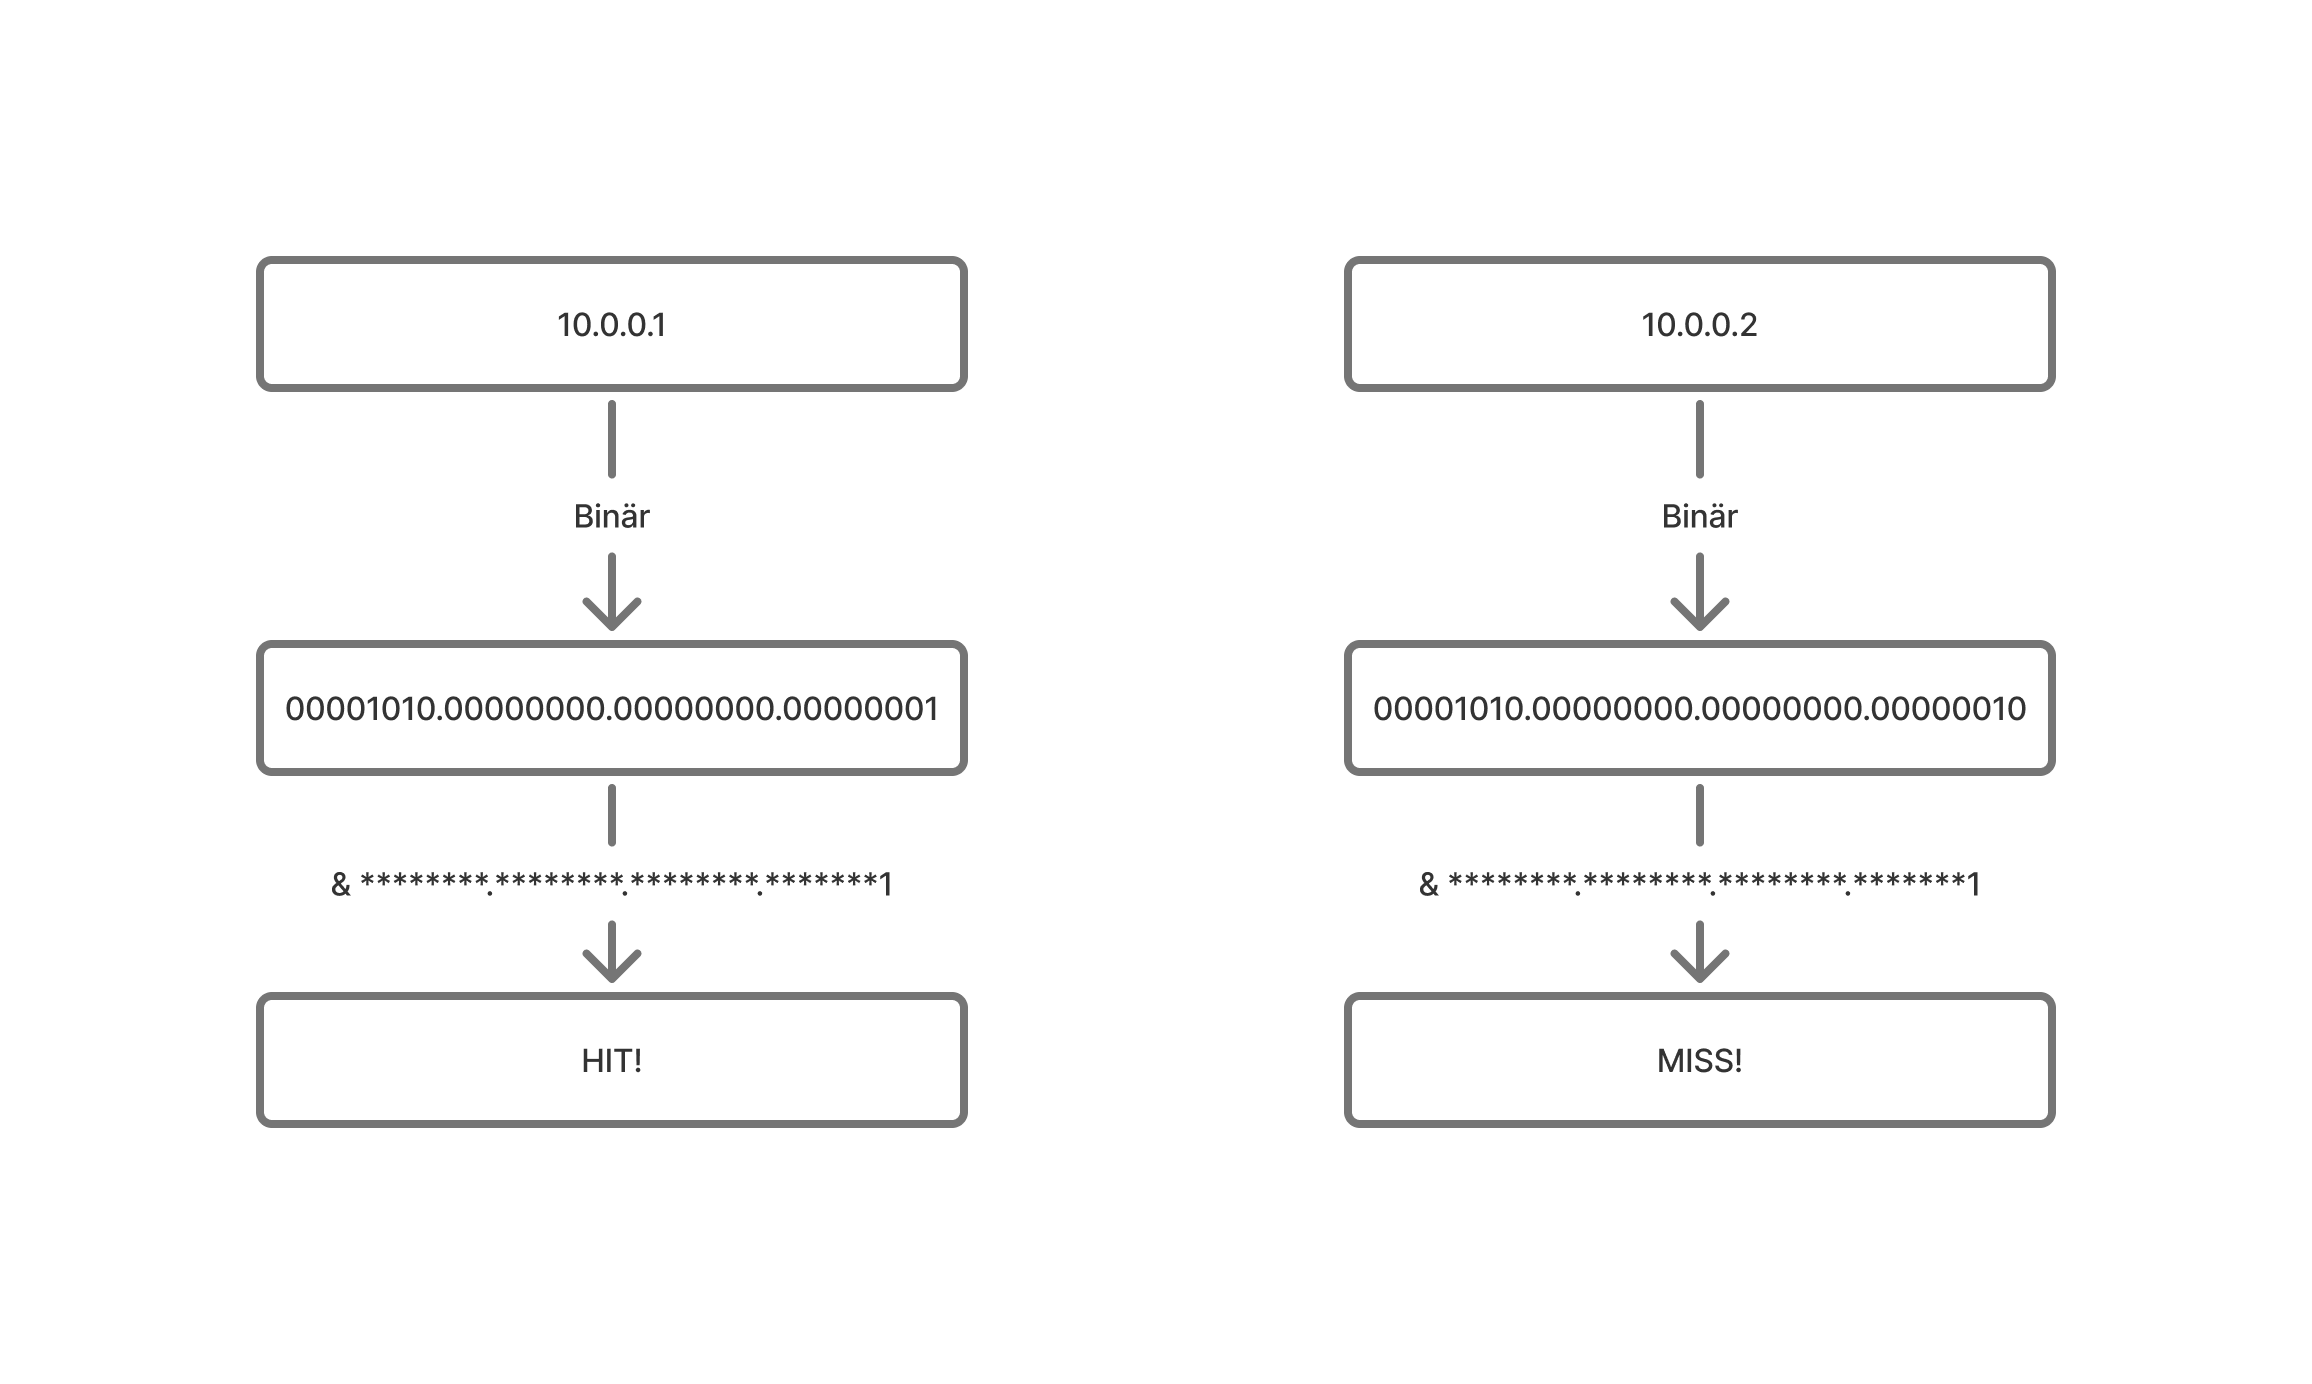
\includegraphics[width=1.1\linewidth]{images/Filter Matching.png}
    \caption{XenoFlow Matching Algorithmus}
    \label{fig:enter-label}
\end{figure}
In Abbildung 6.2 ist ein beispielhafter Aufbau angegeben. Hierbei werden zwei Source-Adressen untersucht. Bei der Adresse 10.0.0.1 ist das letzte Bit der IP gesetzt. Wird also daraufhin der Filter mittels Und-Operator angewendet, so führt diese Adresse zu einem Hit und wird in die entsprechende Pipe eingefügt bzw. von dem entsprechenden Entry verarbeitet. Bei einer IP-Adresse, bei der allerdings das letzte Bit nicht gesetzt ist, wie es bei 10.0.0.2 der Fall ist, wird der Und-Filter das Paket als Miss interpretieren. Der beschriebene Algorithmus beschreibt hier natürlich nur einen Teil, zeigt aber in seinem Aufbau, wie sich anhand leichter Filter zwei Klassen von IP-Adressen erstellen lassen. Genauer in gerade und ungerade IP-Adressen im letzten der 4 Adressfelder. Der große Vorteil dieser Implementierung ist es, dass der Filter vollständig hardwarebeschleunigt arbeiten kann. Es muss somit keinerlei Logik oder ähnliches durchlaufen werden, um die IP-Klassen zu befüllen. Dies sollte sich in den späteren Versuchen deutlich machen.
\subsection{Definition von Backends}
Backends, welche in der Lage sind, Clientanfragen zu bearbeiten und dementsprechend von dem Lastverteiler als valide Endpunkte für eingehenden Verkehr angesehen werden sollen, können in XenoFlow deklarativ definiert werden. Hintergrund dafür ist, dass moderne Systeme wie Kubernetes ebenfalls auf einen deklarativen Konfigurationsstil setzen. Dazu wird die Formatierung \textbf{json} verwendet. 

So können Backends für XenoFlow definiert werden, indem wie folgt JSON-Dateien angelegt werden:
\begin{minted}{json}
{
    "backends": [
        {
            "name": "fips2",
            "mac_address": "A0:88:C2:B5:F4:5A"
        },
        {
            "name": "fips3",
            "mac_address": "E8:EB:D3:9C:71:AC"
        }
    ] 
}
\end{minted}
Dabei spielen die Namen der jeweiligen Backends nur in der Ausgabe von XenoFlow eine Rolle und sind mehr dazu gedacht, bei späteren Weiterentwicklungen von XenoFlow verwendet zu werden. Von größerem Interesse sind die MAC-Adressen, die mit einem jeweiligen Backend assoziiert werden. Diese werden folgend im Lastverteiler verwendet, um eingehende Pakete an diese Adresse weiterzuleiten. Hierbei sei auch erwähnt, dass, ähnlich wie bei DNS-basierten Lastverteilern, im aktuellen Implementierungsstatus nicht sichergestellt ist, ob das jeweilige Backend überhaupt in der Lage ist, Traffic zu verarbeiten. Dies ist allerdings ein Feature, welches sich ebenfalls zu einem späteren Zeitpunkt und unabhängig von dieser Arbeit dazu implementieren lassen würde. Außerdem wäre eine Erweiterung denkbar, die \textbf{yaml} als zusätzliche Markup-Sprache akzeptiert, da YAML wesentlich häufiger in Kontexten wie Kubernetes verwendet wird. Damit wäre XenoFlow ein wenig mehr in line mit modernen Cloudsystemen und deren syntaktischen Entwicklungen.
\newline
Die nun definierten Backends modifizieren die entsprechenden Hardware-Filterregeln. Aufgrund der Natur des gewählten Algorithmus und des binären Zahlensystems ist es im aktuellen Prototypen nur möglich, eine gerade Anzahl von Backends zu deklarieren. Aber auch diese Beschränkung lässt sich durch die Wahl von anderen Netzwerkverkehrsklassifizierungsalgorithmen umgehen. Würde eine Erweiterung hinsichtlich der Health Checks sowie anderer Funktionalitäten wie Logging erfolgen, so ist es dringend angeraten, die allgemeine Architektur der Backendwahl zu modifizieren. Im Rahmen dieser Arbeit wurde die Architektur allerdings bewusst einfach gehalten, um die tatsächliche Leistung der BlueField zu beurteilen und nicht die der entsprechenden Architektur.
\subsection{Open vSwitch}
\begin{figure}
    \centering
    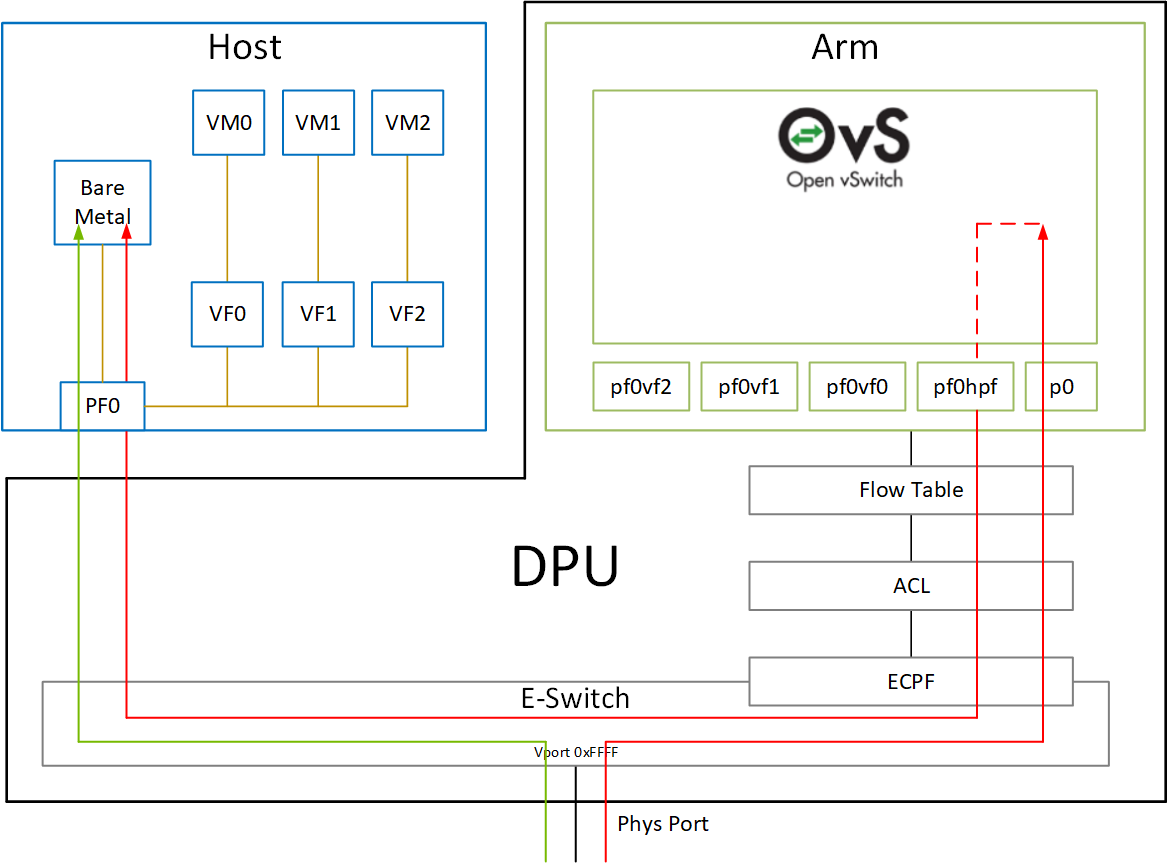
\includegraphics[width=0.85\linewidth]{images/kernel_representors_model.png}
    \caption{Open vSwitch auf der BlueField-3}
    \label{fig:enter-label}
\end{figure}
Die Bluefield verwendet, wie in den vorherigen Kapiteln beschrieben, virtuelle Netzwerkinterfaces, um zwischen dem Host und den ARM-Kernen zu kommunizieren, aber auch, um den Verkehr zwischen den Hardwareport zu steuern. Dazu verwendet NVidia Open vSwitch. Open vSwitch ist eine Applikation, um die Funktionalität eines Switches, der Multilayer arbeiten kann, per Software in Linux abzubilden. Das Projekt wird von der Linux Foundation entwickelt und ist komplett quelloffen unter der Apache-Lizenz 2.0 veröffentlicht. Laut NVidia werden Switch-Regeln, die in Open vSwitch angelegt werden, mittels der ASAP²-Technologie auf die Hardwarebeschleuniger ausgelagert. Dazu ist in Abbildung 6.3 ein Datenpfad von zwei unterschiedlichen Paketen abgezeichnet. Der grüne Pfad zeigt ein Paket, welches direkt vom Switch an den Host hochgereicht wird und dort unter dem Interface PF0 abgeholt werden kann. Das Paket des roten Pfades hingegen durchläuft zunächst den ARM-Kern mit den entsprechenden Interfaces. Unsere Lastverteilung allerdings soll keinen der beiden angegebenen Pfade durchlaufen, sondern lediglich auf den Hardwarebeschleunigern ausgeführt werden. Somit muss allerdings auch deklariert werden, dass eingehender Traffic direkt wieder aus dem entsprechenden anderen Hardwareport ausgegeben wird. Dies ist dank der Erweiterung von OVS von NVidia möglich. Diese Erweiterung trägt den Namen NVIDIA's DOCA-OVS. Im Speziellen soll DOCA-OVS API-Aufrufe ergänzen, die ermöglichen, dass die Hardware entsprechend mit den definierten Regeln arbeiten kann.
\section{Quellcode}
Im folgenden Abschnitt wird ein genauer Überblick über den XenoFlow Lastverteiler gegeben. Es werden die verschiedenen C-Strukturen und Funktionen, die intrinsisch von NVidia bereitgestellt werden, vorgestellt. 
\subsection{main()}
Zu jeder Flow-Applikation gehören nicht nur die entsprechenden Datenstrukturen zur Definition von Pipes und Entries, sondern es müssen auch Konfigurationen allgemeinerer Natur getroffen werden. Diese werden allgemein in einer \_main.c zusammengefasst. In dieser Quellcode-Datei liegt außerdem die eigentliche main Funktion, die zu Beginn eines jeden C Programms ausgeführt wird.
\begin{minted}{c}
int main(int argc, char **argv)
{
	doca_error_t result;
	struct doca_log_backend *sdk_log;
	int exit_status = EXIT_FAILURE;
	struct application_dpdk_config dpdk_config = {
		.port_config.nb_ports = 2,
		.port_config.nb_queues = 4,
		.port_config.nb_hairpin_q = 2,
	};
\end{minted}
Zunächst werden hier einige Datenstrukturen deklariert. Interessant sind hierbei die\newline\texttt{doca\_log\_backend} und \texttt{application\_dpdk\_config} Strukturen.

Das Logbackend wird verwendet, um festzulegen, wie und welches Loglevel erfasst werden soll.
Hierzu wird mit den intrinsischen Funktionsaufrufen
\begin{minted}{c}
result = doca_log_backend_create_standard();
if (result != DOCA_SUCCESS)
    goto sample_exit;
result = doca_log_backend_create_with_file_sdk(stderr, &sdk_log);
if (result != DOCA_SUCCESS)
    goto sample_exit;
result = doca_log_backend_set_sdk_level(sdk_log, DOCA_LOG_LEVEL_WARNING);
if (result != DOCA_SUCCESS)
    goto sample_exit;
\end{minted}
die entsprechende Struktur initialisiert und \texttt{stderr} als Output-Zeiger übergeben. Hier könnten theoretisch auch andere Ziele für die entsprechenden Lognachrichten festgelegt werden. Außerdem wird das minimale Loglevel festgelegt. Lognachrichten, die unter diesem Loglevel liegen, werden nicht angezeigt. Es haben sich hierbei folgende Loglevel entwickelt, die auch in DOCA verwendet werden können:
\begin{itemize}
    \item DEBUG - Sehr verbose und ausführliche Informationen zum auffinden von Fehlern im Betrieb
    \item INFO - Allgemeine Informationen über den Programmstatus
    \item WARNING - Warnungen über eventuell aufkommende Fehler
    \item ERROR - Direkte Fehlermeldungen
\end{itemize}
Eine klassische Lognachricht des Levels INFO sieht wie folgt aus:
\begin{minted}{c}
DOCA_LOG_INFO("Starting the load balancer");
\end{minted}
Als nächstes wird DPDK initialisiert. Dazu wird abermals mittels einer DOCA intrinsischen Funktion die zuvor erstellte Datenstruktur übergeben und außerdem wird der Name, der folgend als ID für die laufende DOCA Applikation verwendet wird, festgelegt:
\begin{minted}{c}
doca_argp_init("doca_flow_lb", NULL);

doca_argp_set_dpdk_program(dpdk_init);

doca_argp_start(argc, argv);
\end{minted}
Mittels des letzten Funktionsaufrufs werden die Parameter der Konsole mit an DOCA übergeben. Dies ist vor allem dazu gebräuchlich, um zu deklarieren, über welches PCI Interface mit der BlueField kommuniziert werden soll, da es möglich ist, mehrere BlueFields in einem Host zu verbauen.
Zuletzt wird nun unsere eigentliche Applikation ausgeführt:
\begin{minted}{c}
xeno_flow(dpdk_config.port_config.nb_queues);
\end{minted}
\subsection{xeno\_flow()}
Als erstes findet die Deklaration sämtliche Datenstrukturen deklariert, die im Folgenden von XenoFlow gebraucht werden:
\begin{minted}{c}
int nb_ports = 1;
struct flow_resources resource = {1};
uint32_t nr_shared_resources[SHARED_RESOURCE_NUM_VALUES] = {0};
struct doca_flow_port *ports[2];
struct doca_dev *dev_arr[nb_ports];
struct doca_flow_pipe *udp_pipe;
int port_id = 0;
uint32_t shared_counter_ids[] = {0, 1};
struct doca_flow_resource_query query_results_array[nb_ports];
struct doca_flow_shared_resource_cfg cfg = {.domain = DOCA_FLOW_PIPE_DOMAIN_DEFAULT};
struct entries_status status;
int num_of_entries = 4;
doca_error_t result;
nr_shared_resources[DOCA_FLOW_SHARED_RESOURCE_COUNTER] = 2;
XenoFlowConfig *config = load_config();
\end{minted}
Hier wird definiert, wie viele Ports von XenoFlow verwendet werden sollen (allerdings nur, wie viele später mit Pipes genutzt werden; es kann auf mehr Ports weitergeleitet werden) und es werden die Strukturen für die späteren Pipedefinitionen festgelegt. Außerdem wird in der letzten Zeile die Konfiguration aus der \texttt{backends.json} geladen. Diese kann dann später vom Lastverteilungsalgorithmus verwendet werden. In DOCA Flow wird ein sehr expliziter Programmierstil gefordert. Es muss stets genau angegeben werden, wie viele Elemente von Strukturen an DOCA übergeben werden. So muss beispielsweise die Anzahl an Entries in den Pipes klar angegeben sein.
\newline
Nun können die eigentlichen Konfigurationsfunktionen aufgerufen werden. Es sei kurz erwähnt, dass die Flow-Beispielapplikationen meist das Errorhandling mittels eines \texttt{if} realisieren. Da dies zu einem enorm langen und teils unleserlichen Quelltext führt, wurde die Funktion \texttt{doca\_try} implementiert, die im Wesentlichen nur den \texttt{return} des Funktionsaufrufs überprüft. Ist dieser != DOCA\_SUCCESS, so wird eine Fehlermeldung ausgegeben. Damit konnte der Quellcode um ca. 100 Zeilen verkürzt werden.
\begin{minted}{c}
DOCA_LOG_INFO("Number of backends: %d", config->numBackends);

doca_try(
    init_doca_flow(
        nb_queues, 
        "vnf,hws", 
        &resource, 
        nr_shared_resources
    ), "Failed to init DOCA Flow", nb_ports, ports
);

doca_try(
    init_doca_flow_ports(
        2, 
        ports, 
        true, 
        dev_arr
    ), "Failed to init DOCA ports", nb_ports, ports
);

doca_try(
    doca_flow_shared_resource_set_cfg(
        DOCA_FLOW_SHARED_RESOURCE_COUNTER, 
        0, 
        &cfg
    ), "Failed to configure shared counter to port", nb_ports, ports
);



doca_try(
    doca_flow_shared_resources_bind(
        DOCA_FLOW_SHARED_RESOURCE_COUNTER, 
        &shared_counter_ids[0], 
        1, 
        ports[0]
    ), "Failed to bind shared counter to pipe", nb_ports, ports
);

\end{minted}
Mittels \texttt{init\_doca\_flow()} wird DOCA Flow initialisiert. Somit wird sichergestellt, dass die API, die mit den Hardwareeinheiten kommuniziert, verfügbar ist und auf kommende Eingaben wartet. Selbiges gilt für \texttt{init\_doca\_flow\_ports()}. Hier werden die entsprechenden beiden Hardwareports an der Netzwerkkarte angewiesen, dass nun Traffic erwartet werden kann, der mittels Steering-Regeln aus DOCA Flow kontrolliert wird. Anschließend werden mittels \texttt{doca\_flow\_shared\_resources\_bind()} die Counter-Ressourcen gebunden. Diese werden im späteren Programmablauf verwendet, um einen Livestatus über die verteilte Last zu erhalten. Diese Ressource muss abermals intrinsisch an DOCA Flow übergeben werden, damit das entsprechende Hardwarebackend angesprochen werden kann.
\begin{minted}{c} 
doca_try(
    create_root_pipe(
        ports[0], 
        0, 
        DOCA_FLOW_L4_TYPE_EXT_UDP, 
        &udp_pipe
    ), "Failed to create pipe", nb_ports, ports
);

doca_try(
    add_shared_counter_pipe_entry(
        udp_pipe, 
        DOCA_FLOW_L4_TYPE_EXT_UDP, 
        shared_counter_ids[0], 
        &status
    ), "Failed to add entry", nb_ports, ports
);

doca_try(
    doca_flow_entries_process(
        ports[0], 
        0, 
        DEFAULT_TIMEOUT_US, 
        num_of_entries
    ), "Failed to process entries", nb_ports, ports
);
\end{minted}
Nun werden die beiden entscheidenden Funktionen \texttt{create\_root\_pipe()} und \newline\texttt{add\_shared\_counter\_pipe\_entry()} aufgerufen. Diese beinhalten die entsprechende Lastverteilungslogik. Zuletzt wird DOCA Flow angewiesen, die angelegten Entries zu verarbeiten. In diesem Schritt findet die eigentliche Hardwareauslagerung statt. Die Funktion dazu lautet \texttt{doca\_flow\_entries\_process()}.
\subsection{Pipe und Entry Erstellung}
\textit{Die folgenden Quellcodeabschnitte wurden aufgrund der besseren Lesbarkeit leicht gekürzt.}
Im folgenden Code ist zunächst die Erstellung einer Pipe, die zunächst sämtlichen Netzwerkverkehr abfängt:
\begin{minted}{c}
static doca_error_t create_root_pipe(
    struct doca_flow_port *port,
    int port_id,
    enum doca_flow_l4_type_ext out_l4_type,
    struct doca_flow_pipe **pipe
) {
    struct doca_flow_match match;
    struct doca_flow_match match_mask;
    struct doca_flow_monitor monitor;
    struct doca_flow_actions actions0, *actions_arr[2];
    struct doca_flow_fwd fwd, fwd_miss;
    struct doca_flow_pipe_cfg *pipe_cfg;
    
    match.outer.l3_type = DOCA_FLOW_L3_TYPE_IP4;
    match.outer.ip4.src_ip = BE_IPV4_ADDR(255, 255, 255, 255);
    match_mask.outer.ip4.src_ip = BE_IPV4_ADDR(0, 0, 0, 1);
    DOCA_LOG_INFO("%d", match_mask.outer.ip4.src_ip);
    
    SET_MAC_ADDR(
        actions0.outer.eth.dst_mac, 
        0xff, 0xff, 0xff, 0xff, 0xff, 0xff
    );
    SET_MAC_ADDR(
        actions0.outer.eth.src_mac, 
        0xff, 0xff, 0xff, 0xff, 0xff, 0xff
    );
    actions_arr[0] = &actions0;
    monitor.counter_type = DOCA_FLOW_RESOURCE_TYPE_SHARED;
    monitor.shared_counter.shared_counter_id = 0xffffffff;
    
    doca_flow_pipe_cfg_create(&pipe_cfg, port);
    set_flow_pipe_cfg(
        pipe_cfg, 
        "SHARED_COUNTER_PIPE", 
        DOCA_FLOW_PIPE_BASIC, 
        true
    );
    doca_flow_pipe_cfg_set_match(pipe_cfg, &match, &match_mask);
    doca_flow_pipe_cfg_set_actions(pipe_cfg, actions_arr, NULL, NULL, 1);
    doca_flow_pipe_cfg_set_monitor(pipe_cfg, &monitor);
    
    fwd.type = DOCA_FLOW_FWD_PORT;
    fwd.port_id = 1;
    fwd_miss.type = DOCA_FLOW_FWD_DROP;
    
    doca_flow_pipe_create(pipe_cfg, &fwd, &fwd_miss, pipe);
}
\end{minted}
Wie schon in Kapitel 3 dem Aufbau einer Pipe zu entnehmen ist, besteht eine Pipe grundsätzlich aus den Elementen \textbf{Match}, \textbf{Monitor}, \textbf{Action} und \textbf{Forward}. Diese werden mittels entsprechender DOCA Flow Structs deklariert und mit den entsprechenden Werten gefüllt. Hierzu sei erwähnt, dass damit alle Bits für das Matching oder eine spätere Action als aktiv geschaltet sein müssen. Sollen sie also im späteren Programmablauf gelesen oder modifiziert werden können, müssen die entsprechenden Bits in der Pipe-Deklaration als 1 gesetzt werden. Dazu sind z.B. die Counter-ID auf \texttt{0xffffffff} oder die src\_mac auf \texttt{0xff, 0xff, 0xff, 0xff, 0xff, 0xff}. Mit der Erstellung der Pipe sollten die entsprechenden Bitfelder auf der Hardware der BlueField-3 aktiviert sein. Außerdem muss, da wir einen impliziten Match forcieren wollen, eine zweite Filtermaske gesetzt werden, die bei Aufruf der intrinsischen Funktion \texttt{doca\_flow\_pipe\_cfg\_set\_match()} mit übergeben wird. Außerdem müssen bereits die \texttt{doca\_flow\_actions} angegeben werden, die in den einzelnen Entries zur Anwendung kommen. Dabei wird nicht spezifiziert, was genau modifiziert werden soll, sondern nur, welche Bitfelder zur Modifikation freigegeben sind.

Zuletzt wird mittels der Funktion \texttt{doca\_flow\_pipe\_create()} die entsprechende Pipe final angelegt. Ist dieser Funktionsaufruf ohne Fehlermeldung und erfolgreich, so ist die Hardwaresteering-Regel aktiv und der Traffic wird nun gemäß den angelegten Regeln verarbeitet.
\newline Da mit der Pipe noch nicht die spezielle Lastverteilung eingebaut ist, sondern lediglich definiert wurde, welche Bitfelder verarbeitet werden sollen und welcher Traffic überhaupt abgegriffen werden soll, ist im folgenden Quelltext die Erstellung der beiden speziellen Entries angegeben:
\begin{minted}{c}
static doca_error_t add_shared_counter_pipe_entry(
    struct doca_flow_pipe *pipe,
    enum doca_flow_l4_type_ext out_l4_type,
    uint32_t shared_counter_id,
    struct entries_status *status
) {
    /**
        ...
    **/
    
    monitor.shared_counter.shared_counter_id = shared_counter_id;
    
    match.outer.ip4.src_ip = BE_IPV4_ADDR(0, 0, 0, 1);	
    actions.action_idx = 0;
    SET_MAC_ADDR(
        actions.outer.eth.dst_mac, 
        0xe8, 0xeb, 0xd3, 0x9c, 0x71, 0xac
    );
    SET_MAC_ADDR(
        actions.outer.eth.src_mac, 
        0xc4, 0x70, 0xbd, 0xa0, 0x56, 0xbd
    );
    doca_flow_pipe_add_entry(
        0, 
        pipe, 
        &match, 
        &actions, 
        &monitor, 
        NULL, 
        0, 
        status, 
        &entry_mac
    );
    /**
        ...
    **/
    return DOCA_SUCCESS;
}
\end{minted}
In diesem letzten, aber auch wichtigsten Codeabschnitt findet der tatsächliche MAC-Adressen-Rewrite statt. Zunächst wird nun der explizite Filterteil auf der Ebene eines einzelnen Entry gesetzt. Dazu erhält die Match-Datenstruktur ein IP-Bitfeld, bei dem nur das letzte Bit gesetzt ist. Das heißt, dieses Entry fängt alle Pakete ab, deren Source-IP-Adresse auf dem letzten Bit eine 1 gesetzt hat. Daraufhin muss die Action ID definiert werden. Diese Action ID wird vor allem zum späteren Logging verwendet, um zu überprüfen, wie viele Pakete von dieser Action verarbeitet wurden. Anschließend sind die entsprechenden MAC-Adressen in der \texttt{actions.outer.eth.dst\_mac} und der \texttt{actions.outer.src\_mac} angegeben.
Mittels \texttt{doca\_flow\_pipe\_add\_entry()} kann nun der entsprechenden Pipe das Entry zugeordnet werden. Das im Code gezeigte Entry ist lediglich eines für ein entsprechendes Backend, dessen MAC-Adresse in der dst\_mac angegeben wird. Sollen nun mehr Backends hinzugefügt werden, benötigt es eine abermalige Ausführung. 
\subsection{Logging und Datenerfassung}
Der XenoFlow Lastverteiler hat eine Echtzeit-Datenerfassung mit implementiert. Dazu wird in einem periodischen Intervall ein 
\begin{minted}{c}
doca_flow_shared_resources_query(
    DOCA_FLOW_SHARED_RESOURCE_COUNTER,
    shared_counter_ids,
    query_results_array,
    nb_ports
);
\end{minted}
Aufruf gemacht. Dessen Ergebnis ist eine Datenstruktur, die einfach ausgelesen werden kann, um die entsprechenden Werte zur Laufzeit auf der Kommandozeile ausgeben zu können.

\subsection{Bemerkung}
Alle Funktionalitäten sind aus dem von NVidia bereitgestellten Headerfile\texttt{ doca\_flow.h} entnommen worden. Die tatsächlichen Implementationen sind \textbf{nicht} quelloffen. Es ist nicht ersichtlich, welche Algorithmen zur Anwendung kamen. Die gegebene Headerdatei ist zwar kommentiert, es wäre allerdings deutlich einfacher, das Projekt quelloffen zu halten, sodass ein genauerer Einblick in die interne Funktionsweise ermöglicht wird. Die Libraries werden als .so-Dateien bereitgestellt.